% LaTeX source for textbook ``How to think like a computer scientist''
% Copyright (c)  2001  Allen B. Downey, Jeffrey Elkner, and Chris Meyers.

% Permission is granted to copy, distribute and/or modify this
% document under the terms of the GNU Free Documentation License,
% Version 1.1  or any later version published by the Free Software
% Foundation; with the Invariant Sections being "Contributor List",
% with no Front-Cover Texts, and with no Back-Cover Texts. A copy of
% the license is included in the section entitled "GNU Free
% Documentation License".

% This distribution includes a file named fdl.tex that contains the text
% of the GNU Free Documentation License.  If it is missing, you can obtain
% it from www.gnu.org or by writing to the Free Software Foundation,
% Inc., 59 Temple Place - Suite 330, Boston, MA 02111-1307, USA.

\chapter{Clases y funciones}
\label{time}
\index{función}
\index{método}


\section{Hora}

Como otro ejemplo de tipo de dato definido por el usuario definiremos
una clase llamada \texttt{Hora}:

\beforeverb
\begin{verbatim}
class Hora:
  pass
\end{verbatim}
\afterverb
%
Ahora podemos crear un nuevo objeto \texttt{Hora} y asignarle atributos
para las horas, minutos y segundos:

\beforeverb
\begin{verbatim}
tiempo = Hora()
tiempo.hora = 11
tiempo.minutos = 59
tiempo.segundos = 30
\end{verbatim}
\afterverb
%
El diagrama para el objeto \texttt{Hora} luce así:

\beforefig
\centerline{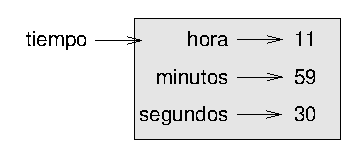
\includegraphics{illustrations/time.eps}}
\afterfig


\section{Funciones puras}
\index{función pura}
\index{tipo función!pura}

En las siguientes secciones escribiremos dos versiones de una
función denominada \texttt{sumarHoras}, que calcule la suma
de dos   \texttt{Horas}. Esto demostrará dos clases de funciones:
las puras y los modificadores.

La siguiente es una versión de  \texttt{sumarHoras}:

\beforeverb
\begin{verbatim}
def sumarHoras(t1, t2):
  sum = Hora()
  sum.hora = t1.hora + t2.hora
  sum.minutos = t1.minutos + t2.minutos
  sum.segundos = t1.segundos + t2.segundos
  return sum
\end{verbatim}
\afterverb
%
La función crea un nuevo objeto  \texttt{Hora}, inicializa
sus atributos y retorna una referencia hacia el nuevo objeto.
Esto se denomina {\bf función pura}, porque no modifica ninguno
de los objetos que se le pasaron como parámetro ni tiene
efectos laterales, como desplegar un valor o leer entrada
del usuario.

Aquí hay un ejemplo de uso de esta función. Crearemos dos
objetos  {\tt Hora}: \texttt{horaPan}, que contiene el tiempo que le toma a un panadero
hacer pan y \texttt{horaActual}, que contiene la hora actual. Luego usaremos \texttt{sumarHoras} para averiguar
a qué hora estará listo el pan. Si no ha terminado la función {\tt
imprimirHora} aún, adelántese a la Sección~\ref{printTime} antes
de intentar esto:

\beforeverb
\begin{verbatim}
>>> horaActual = Hora()
>>> horaActual.hora = 9
>>> horaActual.minutos = 14
>>> horaActual.segundos =  30

>>> horaPan = Hora()
>>> horaPan.hora =  3
>>> horaPan.minutos =  35
>>> horaPan.segundos =  0

>>> horaComer = sumarHoras(horaActual, horaPan)
>>> imprimirHora(horaComer)
\end{verbatim}
\afterverb
%
La salida de este programa es \texttt{12:49:30}, que está correcta. Por
otro lado, hay casos en los que no funciona bien. ¿Puede pensar en uno?

El problema radica en que esta función no considera los casos donde
el número de segundos o minutos suman más de sesenta. Cuando eso 
ocurre tenemos que  ``acarrear'' los segundos extra a la columna
de  minutos. También puede pasar lo mismo con los minutos.

Aquí hay una versión correcta:

%\beforeverb
\begin{verbatim}
def sumarHoras(t1, t2):
  sum = Hora()
  sum.hora = t1.hora + t2.hora
  sum.minutos = t1.minutos + t2.minutos
  sum.segundos = t1.segundos + t2.segundos

  if sum.segundos >= 60:
    sum.segundos = sum.segundos - 60
    sum.minutos = sum.minutos + 1

  if sum.minutos >= 60:
    sum.minutos = sum.minutos - 60
    sum.hora = sum.hora + 1

  return sum
\end{verbatim}
%\afterverb

Aunque ahora ha quedado correcta, ha empezado a agrandarse. Más
adelante sugeriremos un enfoque alternativo que produce un código
más corto.


\section{Modificadoras}
\label{increment}
\index{modificadora}
\index{tipo función!modificadora}

A veces es deseable que  una función modifique uno o varios
de los objetos que recibe como parámetros. Usualmente, el 
código que hace el llamado a la función conserva una referencia a los
objetos que está pasando, así que cualquier cambio que la
función les haga será evidenciado por dicho código.
Este tipo de funciones se denominan {\bf modificadoras}.

\texttt{incrementar}, que agrega un número de segundos
a un objeto \texttt{Hora}, se escribiría más naturalmente
como función modificadora. Un primer acercamiento a la 
función luciría así:

%\adjustpage{-2}
%\pagebreak

%\beforeverb
\begin{verbatim}
def incrementar(h, segundos):
  h.segundos = h.segundos + segundos

  if h.segundos >= 60:
    h.segundos = h.segundos - 60
    h.minutos = h.minutos + 1

  if h.minuto >= 60:
    h.minutos = h.minutos - 60
    h.hora = h.hora + 1

  return h
\end{verbatim}
%\afterverb
%
La primera línea ejecuta la operación básica, las siguientes
consideran los casos especiales que ya habíamos visto.

¿Es correcta esta función? ¿Que pasa si el parámetro
 \texttt{segundos} es mucho más grande que sesenta?
 En ese caso, no sólo es suficiente añadir uno, tenemos
que sumar de uno en uno hasta que  \texttt{segundos} sea
menor que sesenta.
Una solución consiste en reemplazar las sentencias  \texttt{if}  por sentencias \texttt{while}:

\beforeverb
\begin{verbatim}
def incrementar(hora, segundos):
  hora.segundos = hora.segundos + segundos

  while hora.segundos >= 60:
    hora.segundos = hora.segundos - 60
    hora.minutos = hora.minutos + 1

  while hora.minutos >= 60:
    hora.minutos = hora.minutos - 60
    hora.hora = hora.hora + 1

  return hora

  time.segundos = time.segundos + segundos

\end{verbatim}
\afterverb
%
Ahora, la función sí es correcta, aunque no sigue el proceso
 más eficiente. 

\section{¿Cual es el mejor estilo?}
\index{estilo de programación funcional}

%\adjustpage{1}

Todo lo que puede hacerse con modificadoras también se 
puede hacer con funciones puras. De hecho, algunos lenguajes
de programación sólo permiten funciones puras. La evidencia
apoya la tesis de que los programas que usan solamente 
funciones puras se desarrollan más rápido y son menos
propensos a errores que los programas que usan modificadoras.
Sin embargo, las funciones modificadoras, a menudo, son 
convenientes y, a menudo, los programas funcionales puros
son menos eficientes.

En general, le recomendamos que escriba funciones puras 
cada vez que sea posible y recurrir a las modificadoras
solamente si hay una ventaja en usar este enfoque. Esto
se denomina un {\bf estilo de programación funcional}.


\section{Desarrollo con prototipos vs. planificación}
\label{convert}
\index{desarrollo con prototipos}

En este capítulo mostramos un enfoque de desarrollo de 
programas que denominamos  {\bf desarrollo con prototipos}. 
Para cada problema escribimos un bosquejo  (o prototipo) que
ejecutará el cálculo básico y lo probará en unos cuantos
casos de prueba, corrigiendo errores a medida que surgen.

Aunque este enfoque puede ser efectivo, puede conducirnos
a código innecesariamente complicado ---ya que considera
muchos casos especiales---y poco confiable---ya que es
difícil asegurar que hemos descubierto todos los errores.

Una alternativa es el {\bf desarrollo planificado}, en 
el que la profundización en el dominio del problema puede
darnos una comprensión profunda que facilita bastante la 
programación. En el caso anterior, comprendimos que 
un objeto  \texttt{Hora} realmente es un número de
tres dígitos en base 60!  El componente \texttt{segundos} 
contiene las  ``unidades,'' el componente
\texttt{minutos} la  ``columna de sesentas,'' y 
el componente \texttt{hora} contiene la ``columna de tres mil 
seiscientos.''

Cuando escribimos  \texttt{sumarHoras} e \texttt{incrementar}, 
realmente estábamos haciendo una suma en base 60, razón 
por la cual teníamos que efectuar un acarreo de una columna
a la siguiente.

Esta observación sugiere otro enfoque al problema---podemos
convertir un objeto  \texttt{Hora} en un número único 
y aprovecharnos del hecho de que el computador sabe
realizar aritmética.  La siguiente función convierte
un objeto  \texttt{Hora} en un entero:

\beforeverb
\begin{verbatim}
def convertirASegundos(t):
  minutos = t.hora * 60 + t.minutos
  segundos = minutos * 60 + t.segundos
  return segundos
\end{verbatim}
\afterverb
%
Ahora necesitamos una forma de convertir desde entero
a un objeto  \texttt{Hora}:

\adjustpage{1}

\beforeverb
\begin{verbatim}
def crearHora(segundos):
  h = Hora()
  h.hora = segundos/3600
  segundos = segundos - h.hora * 3600
  h.minutos = segundos/60
  segundos = segundos - h.minutos * 60
  h.segundos = segundos
  return h
\end{verbatim}
\afterverb
%
Usted debe pensar unos minutos para convencerse de que
esta técnica sí convierte, de una base a otra, correctamente.
Asumiendo que ya está convencido, se pueden usar las 
funciones anteriores para reescribir {\tt sumarHoras}:

\beforeverb
\begin{verbatim}
def sumarHoras(t1, t2):
  segundos = convertirASegundos(t1) + convertirASegundos(t2)
  return crearHora(segundos)
\end{verbatim}
\afterverb
%
Esta versión es mucho más corta que la original, y es mucho
más fácil de demostrar que es correcta (asumiendo, como de 
costumbre, que las funciones que llama son correctas).



\section{Generalización}
\index{generalización}

Desde cierto punto de vista, convertir de base 60
a base 10 y viceversa es más difícil que calcular
solamente con horas. La conversión de bases es más
abstracta, mientras que nuestra intuición para 
manejar horas está más desarrollada.

Pero si tenemos la intuición de tratar las horas como
números en base 60 y hacemos la inversión de escribir
las funciones de conversión  ({\tt convertirASegundos} y 
\texttt{crearHora}), obtenemos un programa más corto,
legible, depurable y confiable.

También facilita la adición de más características. Por
ejemplo, piense en el problema de restar dos  \texttt{Hora}s para
averiguar el tiempo que transcurre entre ellas.  La solución
ingenua haría resta llevando préstamos. En cambio, usar las
funciones de conversión sería mas fácil.

Irónicamente, algunas veces el hacer de un problema algo
más difícil (o más general) lo hace más fácil (porque
hay menos casos especiales y menos oportunidades para
caer en errores).


\section{Algoritmos}
\index{algoritmo}

Cuando usted escribe una solución general para una clase de problemas,
en vez de encontrar una solución específica a un solo problema, ha
escrito un  {\bf algoritmo}. Mencionamos esta palabra antes, pero no 
la definimos cuidadosamente. No es fácil de definir, así que intentaremos
dos enfoques.

Primero, considere algo que no es un algoritmo. Cuando usted aprendió 
a multiplicar dígitos, probablemente memorizó la tabla de multiplicación.
De hecho, usted memorizó 100 soluciones específicas. Este tipo de conocimiento
no es algorítmico.

Pero si usted fuera ``perezoso,'' probablemente aprendió a hacer trampa
por medio de algunos trucos. Por ejemplo, para encontrar el producto entre
$n$ y 9, usted puede escribir  $n-1$ como el primer dígito y $10-n$ como el 
segundo. Este truco es una solución general para multiplicar cualquier 
dígito por el 9. ¡Este es un algoritmo!

Similarmente, las técnicas que aprendió para hacer suma con acarreo ( 
llevando para la columna hacia la derecha), resta con préstamos, y 
división larga, todas son algoritmos. Una de las características
de los algoritmos es que no requieren inteligencia para ejecutarse.
Son procesos mecánicos en el que cada paso sigue al anterior
de acuerdo con un conjunto de reglas sencillas.

En nuestra opinión, es vergonzoso que los seres humanos pasemos
tanto tiempo en la escuela aprendiendo a ejecutar algoritmos que, 
literalmente, no requieren inteligencia.

Por otro lado, el proceso de diseñar algoritmos es interesante,
intelectualmente desafiante y una parte central de lo que 
denominamos programación.

Algunas cosas que la gente hace naturalmente sin dificultad o 
pensamiento consciente, son las mas difíciles de expresar algorítmicamente.
Entender el lenguaje natural es una de ellas. Todos lo hacemos, pero
hasta ahora nadie ha sido capaz de explicar {\em como} lo hacemos, al menos
no con un algoritmo.


\section{Glosario}

\begin{description}

\item[Función pura:] función que no modifica ninguno de los objetos
que recibe como parámetros. La mayoría de las funciones puras son 
fructíferas.

\item[Modificadora:] función que cambia uno o varios de los objetos
que recibe como parámetros. La mayoría de los modificadoras no retornan
nada.

\item[Estilo de programación funcional] estilo de diseño de programas en 
el que la mayoría de funciones son puras.

\item[Desarrollo con prototipos:] es la forma de desarrollar programas empezando
con un prototipo que empieza a mejorarse y probarse gradualmente.

\item[Desarrollo planeado:] es la forma de desarrollar programas que implica
un conocimiento de alto nivel sobre el problema y mas planeación que
el desarrollo incremental o el desarrollo con prototipos.

\item[Algoritmo:]  conjunto de instrucciones para resolver una clase de
problemas por medio de un proceso mecánico, no inteligente.

\index{función pura}
\index{modificadora}
\index{estilo de programació funcional}
\index{desarrollo incremental}
\index{desarrollo!incremental}
\index{desarrollo planeado}
\index{desarrollo!planeado}
\index{algoritmo}

\end{description}

\section{Ejercicios}
\begin{enumerate}

\item Reescriba la función \texttt{incrementar} 
de forma que no contenga ciclos y siga siendo correcta.

\item Reescriba \texttt{incrementar} usando 
convertirASegundos y crearHora.

\item Reescriba \texttt{incrementar} como una función 
pura, y escriba llamados a funciones de las dos versiones.

\item Escriba una función  \texttt{imprimirHora} que reciba
un objeto \texttt{Hora} como argumento y lo imprima de la forma
 \texttt{horas:minutos:segundos}.

\item Escriba una  función booleana \texttt{despues} que reciba dos
objetos \texttt{Hora}, \texttt{t1} y \texttt{t2} como argumentos, y 
retorne cierto si  \texttt{t1} va después de \texttt{t2} cronológicamente
y falso en caso contrario.

\end{enumerate}
